\newpage
\thispagestyle{empty}
% Adicione o TikZ para desenhar a linha vertical
\begin{tikzpicture}[remember picture, overlay]
    \draw[line width=3.4cm, base] ($(current page.north east) - (0,0)$) -- ($(current page.south east) - (0,0)$);
\end{tikzpicture}

\vspace{-1cm} % Espaço vertical para mover a figura para cima e caber na página (ajuste de acordo com o modelo, mantendo na página com uma linha vertical de cor referente a base)
\noindent % Evita indentação
\begin{minipage}{7.7cm}% Define a largura da minipage igual à largura da figura
\protect\vspace{16.5cm}% Ajuste fino para mover nota verticalmente
  \large{{\bfseries\sffamily Nota do autor:} \sffamily Os outros personagens que aparecem nesta tirinha são o Prof. Cloro e Estrôncio, que também estão em outras tirinhas de minha criação. Aqui, apresenta-se a origem do Sir Apple em uma coletânea de tirinhas especiais. A história continua...}
\end{minipage}
\hspace*{\fill} % Empurra a figura para a direita (caso não use a nota do autor então evite pular linha entre o \end{tikzpicture} da linha vertical e \hspace*{\fill} )
% Tirinha 
\begin{minipage}{9cm} % Define a largura da minipage igual à largura da figura
    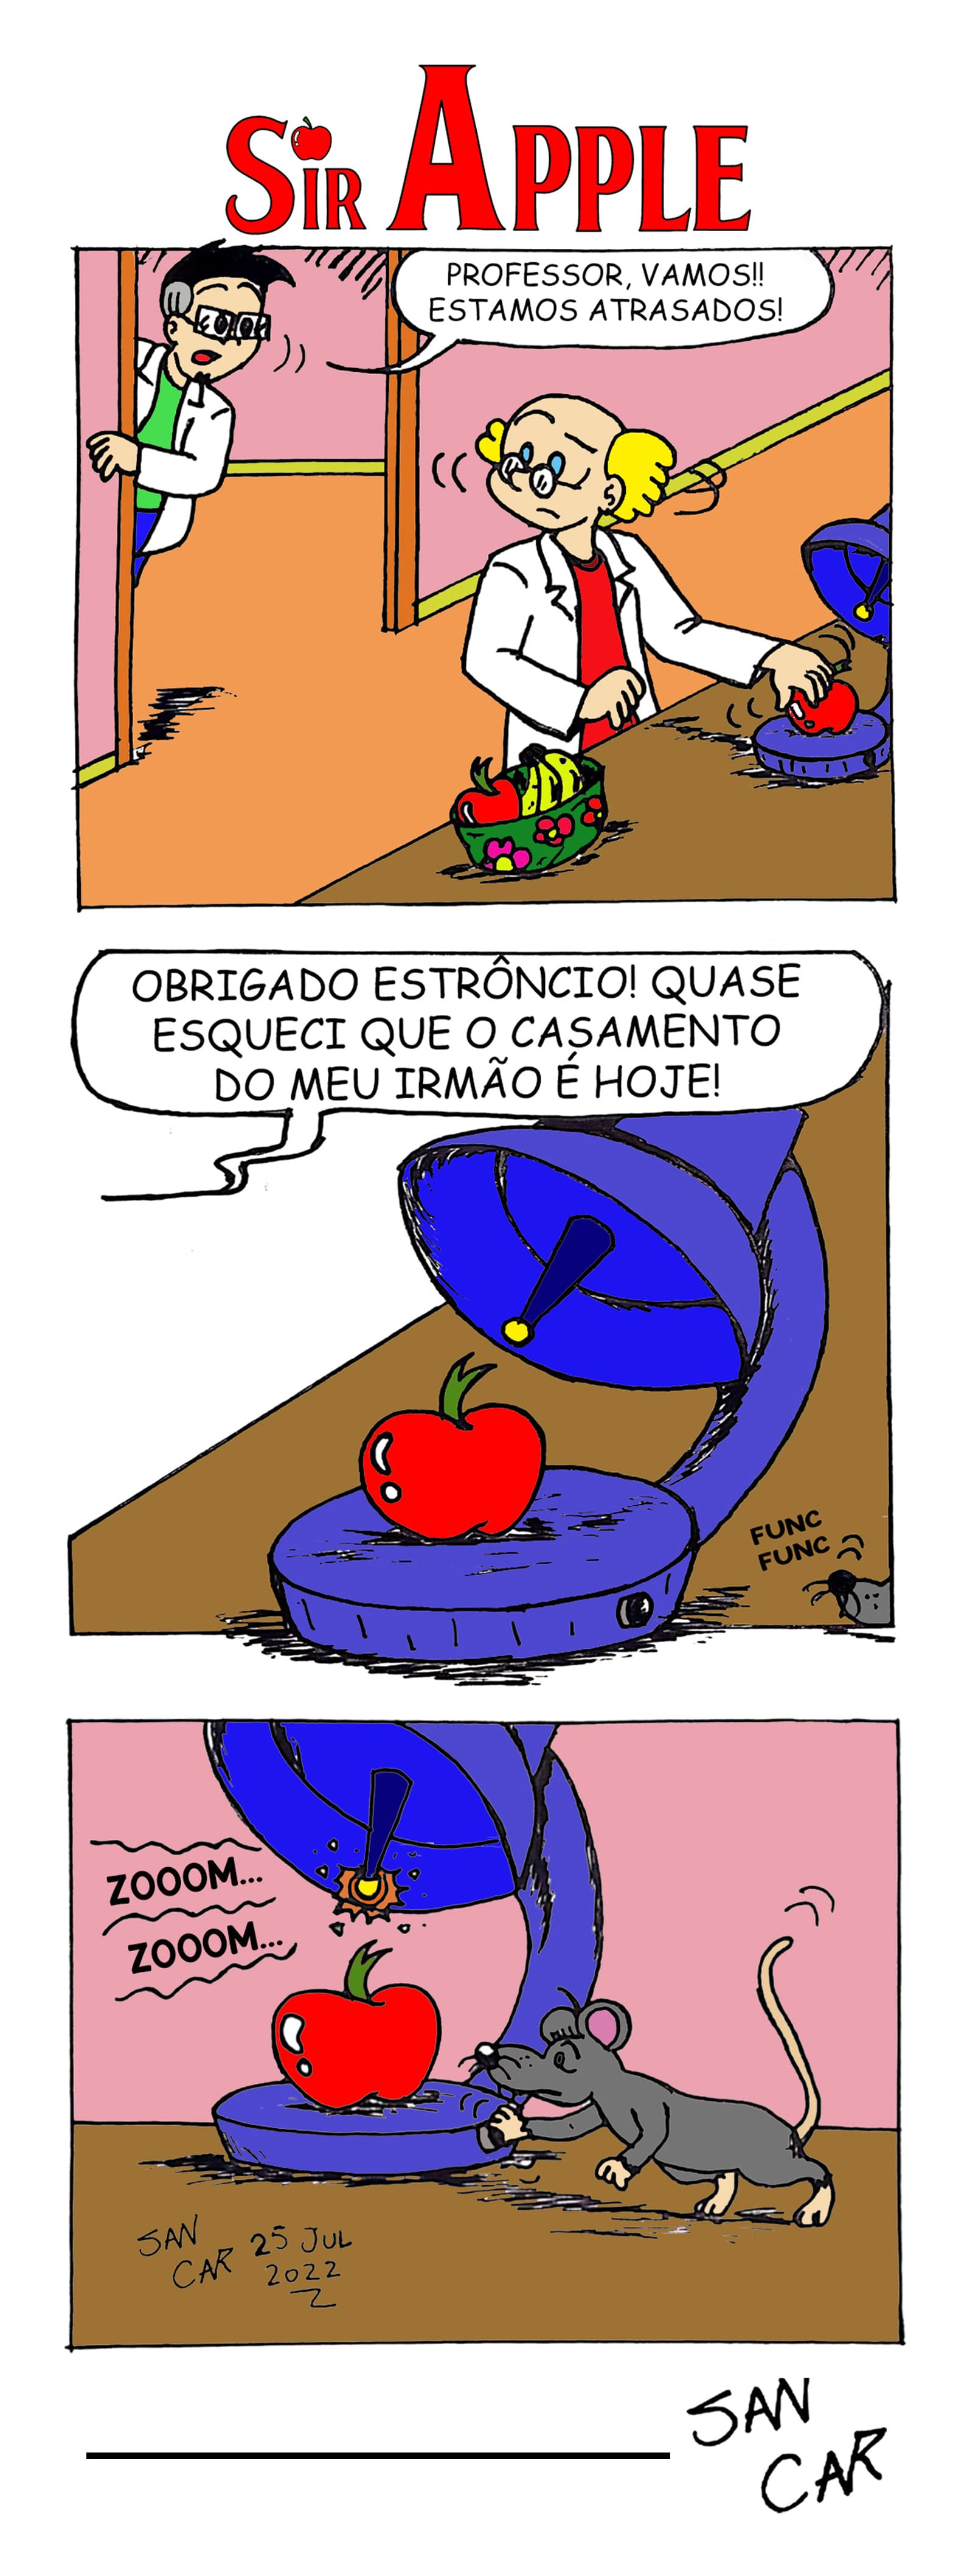
\includegraphics[width=\textwidth]{Tirinha/Tirinha_Fig/Tirinha_Sir_Apple.jpg}
\end{minipage}










